%\documentclass[border={1cm 1cm 1cm 1cm}]{standalone}  %E,S,W,N
\documentclass{scrartcl}

\usepackage{amssymb}
\usepackage{amsmath}
\usepackage{tikz}
\usetikzlibrary{calc}	%for calculations
\pagenumbering{gobble}	%no page number

\begin{document}
	
	%NOTES ON THE \d PARAMETER
	%5 circles: \i+1 best
	%6 circles: \i+2 best (for \i+1, no effect)
	%7 circles: \i+1 best
	%8 circles: \i+1 and \i+3 both look nice
	
	\raisebox{0.5cm}{
	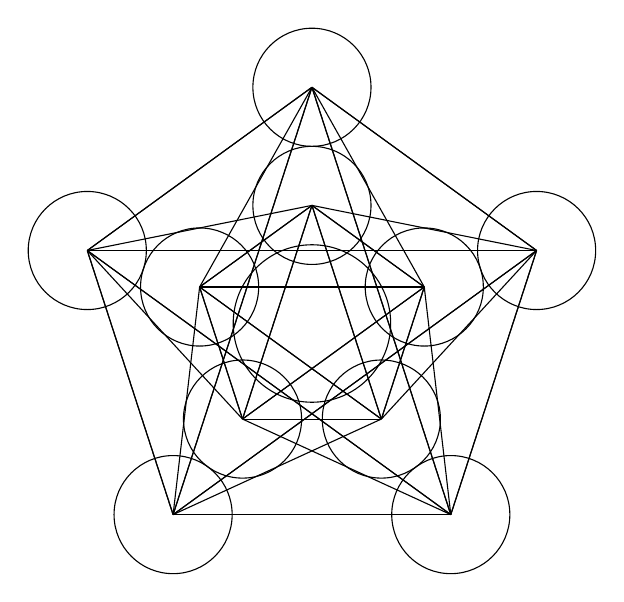
\begin{tikzpicture}%[semithick]
	\def\n{5}	%number of surrounding circles (original: 6)
	\def\s{.75}	%size of circle (original: 1); don't forget to adjust line thickness
	\def\d{1}	%distance connecting outer circles to inner circles (original: 2)
				%in general: \d gives same result as \n/2+\d
	\draw (0,0) circle (1cm);			%central circle
	
	\foreach \i in {1,...,\n}{
		\draw ({2*\s*cos(90+\i*360/\n)},{2*\s*sin(90+\i*360/\n)}) circle (\s cm);
		\draw ({4*\s*cos(90+\i*360/\n)},{4*\s*sin(90+\i*360/\n)}) circle (\s cm);
		\draw ({4*\s*cos(90+\i*360/\n)},{4*\s*sin(90+\i*360/\n)}) -- ({2*\s*cos(90+(\i+\d)*360/\n)},{2*\s*sin(90+(\i+\d)*360/\n)}); %outer circles--inner, left
		\draw ({4*\s*cos(90+\i*360/\n)},{4*\s*sin(90+\i*360/\n)}) -- ({2*\s*cos(90+(\i-\d)*360/\n)},{2*\s*sin(90+(\i-\d)*360/\n)}); %outer--inner, right
		\foreach \j in {1,...,\n}{
			\draw ({4*\s*cos(90+\i*360/\n)},{4*\s*sin(90+\i*360/\n)}) -- ({4*\s*cos(90+(\i+\j)*360/\n)},{4*\s*sin(90+(\i+\j)*360/\n)}); %lines linking outer circles
			\draw ({2*\s*cos(90+\i*360/\n)},{2*\s*sin(90+\i*360/\n)}) -- ({2*\s*cos(90+(\i+\j)*360/\n)},{2*\s*sin(90+(\i+\j)*360/\n)}); %lines linking inner circles
		}
	}			
	\end{tikzpicture}
		} %end raisebox
	%
	%
	\hspace{0.5cm}%
	%
	%
	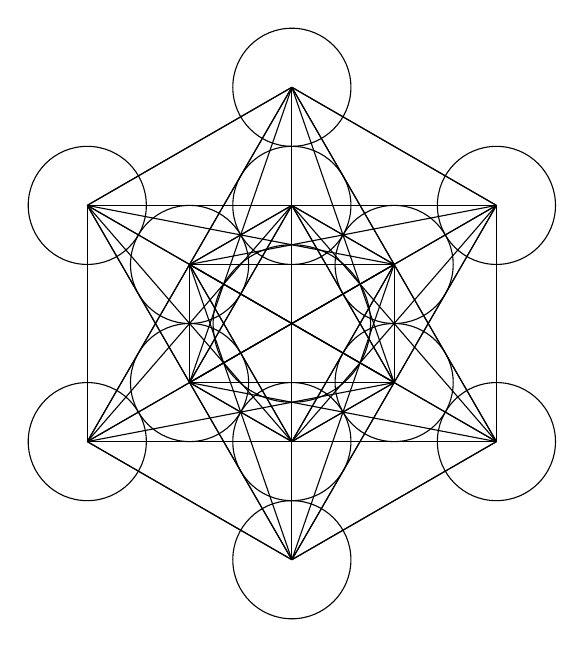
\begin{tikzpicture}%[semithick]
	\def\n{6}	%number of surrounding circles (original: 6)
	\def\s{.75}	%size of circle (original: 1); don't forget to adjust line thickness
	\def\d{2}	%distance connecting outer circles to inner circles (original: 2)
				%in general: \d gives same result as \n/2+\d
	\draw (0,0) circle (1cm);			%central circle
	
	\foreach \i in {1,...,\n}{
	\draw ({2*\s*cos(90+\i*360/\n)},{2*\s*sin(90+\i*360/\n)}) circle (\s cm);
	\draw ({4*\s*cos(90+\i*360/\n)},{4*\s*sin(90+\i*360/\n)}) circle (\s cm);
	\draw ({4*\s*cos(90+\i*360/\n)},{4*\s*sin(90+\i*360/\n)}) -- ({2*\s*cos(90+(\i+\d)*360/\n)},{2*\s*sin(90+(\i+\d)*360/\n)}); %outer circles--inner, left
	\draw ({4*\s*cos(90+\i*360/\n)},{4*\s*sin(90+\i*360/\n)}) -- ({2*\s*cos(90+(\i-\d)*360/\n)},{2*\s*sin(90+(\i-\d)*360/\n)}); %outer--inner, right
	\foreach \j in {1,...,\n}{
		\draw ({4*\s*cos(90+\i*360/\n)},{4*\s*sin(90+\i*360/\n)}) -- ({4*\s*cos(90+(\i+\j)*360/\n)},{4*\s*sin(90+(\i+\j)*360/\n)}); %lines linking outer circles
		\draw ({2*\s*cos(90+\i*360/\n)},{2*\s*sin(90+\i*360/\n)}) -- ({2*\s*cos(90+(\i+\j)*360/\n)},{2*\s*sin(90+(\i+\j)*360/\n)}); %lines linking inner circles
		}
	}			
	\end{tikzpicture}
	
	\vspace{0.5cm}
	
	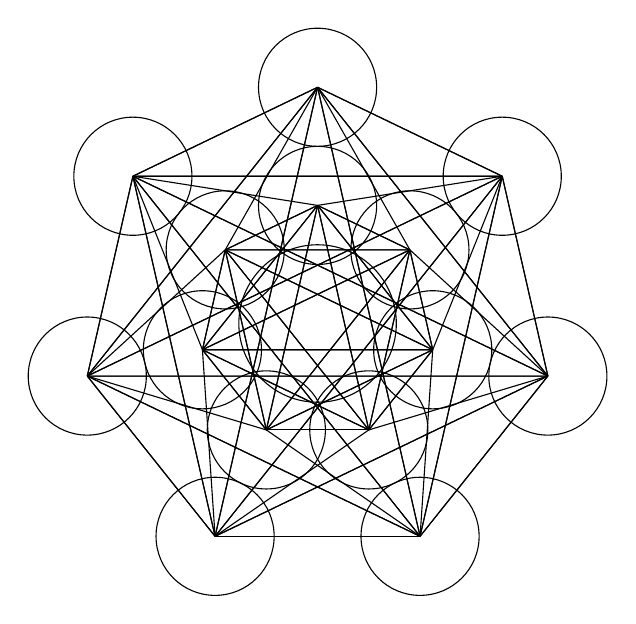
\begin{tikzpicture}%[semithick]
	\def\n{7}	%number of surrounding circles (original: 6)
	\def\s{.75}	%size of circle (original: 1); don't forget to adjust line thickness
	\def\d{1}	%distance connecting outer circles to inner circles (original: 2)
				%in general: \d gives same result as \n/2+\d
	\draw (0,0) circle (1cm);			%central circle
	
	\foreach \i in {1,...,\n}{
		\draw ({2*\s*cos(90+\i*360/\n)},{2*\s*sin(90+\i*360/\n)}) circle (\s cm);
		\draw ({4*\s*cos(90+\i*360/\n)},{4*\s*sin(90+\i*360/\n)}) circle (\s cm);
		\draw ({4*\s*cos(90+\i*360/\n)},{4*\s*sin(90+\i*360/\n)}) -- ({2*\s*cos(90+(\i+\d)*360/\n)},{2*\s*sin(90+(\i+\d)*360/\n)}); %outer circles--inner, left
		\draw ({4*\s*cos(90+\i*360/\n)},{4*\s*sin(90+\i*360/\n)}) -- ({2*\s*cos(90+(\i-\d)*360/\n)},{2*\s*sin(90+(\i-\d)*360/\n)}); %outer--inner, right
		\foreach \j in {1,...,\n}{
			\draw ({4*\s*cos(90+\i*360/\n)},{4*\s*sin(90+\i*360/\n)}) -- ({4*\s*cos(90+(\i+\j)*360/\n)},{4*\s*sin(90+(\i+\j)*360/\n)}); %lines linking outer circles
			\draw ({2*\s*cos(90+\i*360/\n)},{2*\s*sin(90+\i*360/\n)}) -- ({2*\s*cos(90+(\i+\j)*360/\n)},{2*\s*sin(90+(\i+\j)*360/\n)}); %lines linking inner circles
		}
	}			
	\end{tikzpicture}%
	%
	%
	\hspace{0.5cm}%
	%
	%
	\raisebox{-0.35cm}{
	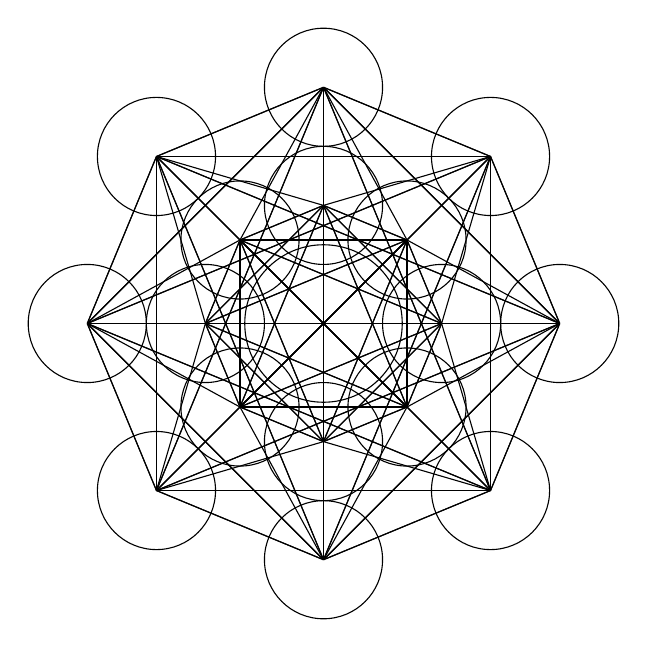
\begin{tikzpicture}%[semithick]
	\def\n{8}	%number of surrounding circles (original: 6)
	\def\s{.75}	%size of circle (original: 1); don't forget to adjust line thickness
	\def\d{1}	%distance connecting outer circles to inner circles (original: 2)
				%in general: \d gives same result as \n/2+\d
	\draw (0,0) circle (1cm);			%central circle
	
	\foreach \i in {1,...,\n}{
		\draw ({2*\s*cos(90+\i*360/\n)},{2*\s*sin(90+\i*360/\n)}) circle (\s cm);
		\draw ({4*\s*cos(90+\i*360/\n)},{4*\s*sin(90+\i*360/\n)}) circle (\s cm);
		\draw ({4*\s*cos(90+\i*360/\n)},{4*\s*sin(90+\i*360/\n)}) -- ({2*\s*cos(90+(\i+\d)*360/\n)},{2*\s*sin(90+(\i+\d)*360/\n)}); %outer circles--inner, left
		\draw ({4*\s*cos(90+\i*360/\n)},{4*\s*sin(90+\i*360/\n)}) -- ({2*\s*cos(90+(\i-\d)*360/\n)},{2*\s*sin(90+(\i-\d)*360/\n)}); %outer--inner, right
		\foreach \j in {1,...,\n}{
			\draw ({4*\s*cos(90+\i*360/\n)},{4*\s*sin(90+\i*360/\n)}) -- ({4*\s*cos(90+(\i+\j)*360/\n)},{4*\s*sin(90+(\i+\j)*360/\n)}); %lines linking outer circles
			\draw ({2*\s*cos(90+\i*360/\n)},{2*\s*sin(90+\i*360/\n)}) -- ({2*\s*cos(90+(\i+\j)*360/\n)},{2*\s*sin(90+(\i+\j)*360/\n)}); %lines linking inner circles
		}
	}			
	\end{tikzpicture}
		}	%end raisebox
	
\end{document}